\documentclass[8pt, a4paper]{article}

%\usepackage{blindtext}
\usepackage{savetrees}
\usepackage{graphicx}
\graphicspath{ {./images/} }

\title{X-Ray Lab Graphs}
\author{Jack Symonds}
\date{}

\begin{document}

\maketitle
\begin{verbatim}
import numpy as np
import matplotlib.pyplot as plt
import scipy.signal as sig

class XrayData:
    def __init__(self, filename):
        with open(filename, 'r', errors='ignore') as df:
            rawlines = df.readlines()
            bm = float(rawlines[4].split(' ')[0])
            bM = float(rawlines[4].split(' ')[1])
            bs = float(rawlines[4].split(' ')[3])
            self.counts = np.array([])
            for line in range(18,len(rawlines)-11):
                self.counts = np.append(self.counts, float(rawlines[line].split()[0]))
            self.angles = np.array([])
            for i in range(0, len(self.counts)):
                self.angles = np.append(self.angles, bm+i*bs)
        self.fig, self.ax = plt.subplots()
        
    def plot(self,height,extraPeaks=[]):
        self.ax.plot(self.angles, self.counts)
        self.ax.set_ylim(0,1.01*np.max(self.counts))
        self.ax.set_ylabel(r'counts per second $R$')
        self.ax.set_xlim(0, np.max(self.angles))
        self.ax.set_xlabel(r'angle of incidence $\theta$')
        plt.subplots_adjust(bottom=0.2)

        scipeaki = sig.find_peaks(self.counts, height=height)[0]

        peaks = []
        for i in scipeaki:
            peaks.append([self.angles[i], self.counts[i]])
        for peak in extraPeaks:
            ind = np.searchsorted(self.angles, peak)
            peaks.append([peak, self.counts[ind]])
        self.peaks = np.array(peaks)

        for peak in self.peaks:
            self.ax.axvline(peak[0], linestyle='--', linewidth=0.5, c='red')
            self.ax.axhline(peak[1], linestyle='--', linewidth=0.5, c='red')

        self.ax.set_xticks(self.peaks[:,0])
        plt.setp(self.ax.get_xticklabels(), rotation=45, rotation_mode='anchor', ha='right')
        self.ax.set_yticks(self.peaks[:,1])

    def get_wavelengths(self, spacing):
        self.wvlengths = np.array([])
        i = 0
        for peak in self.peaks:
            wavelength = 2*spacing*np.sin(peak[0]*(np.pi/180))
            wvlength = "{:.3e}".format(wavelength)
            self.wvlengths = np.append(self.wvlengths, wvlength)
            i +=1
            self.ax.text(peak[0], peak[1]-20, r'$\lambda_{} =$'.format(i) + str(wvlength))
        


scan1 = XrayData('xraydata/LiF1.csv')
scan1.ax.set_title('LiF Count Rate for Bragg Angles')
scan1.plot(220, [31.9])
lifs = 4.02*10**(-10)
scan1.get_wavelengths(lifs)
scan1.fig.savefig('./images/LiF1')
plt.show()

scan2 = XrayData('xraydata/venergy1.csv')
scan2.ax.set_title('LiF Scan with 35 kV Acc. Voltage')
scan2.plot(220)
scan2.get_wavelengths(lifs)
scan2.fig.savefig('./images/ve1')
plt.close()

scan3 = XrayData('xraydata/venergy2.csv')
scan3.ax.set_title('LiF Scan with 30 kV Acc. Voltage')
scan3.plot(150)
scan3.get_wavelengths(lifs)
scan3.fig.savefig('./images/ve2')
plt.close()

scan4 = XrayData('xraydata/venergy3.csv')
scan4.ax.set_title('LiF Scan with 25 kV Acc. Voltage')
scan4.plot(70)
scan4.get_wavelengths(lifs)
scan4.fig.savefig('./images/ve3')
plt.close()

scan5 = XrayData('xraydata/venergy4.csv')
scan5.ax.set_title('LiF Scan with 10 kV Acc. Voltage')
scan5.ax.scatter(scan5.angles, scan5.counts, marker='.', color='brown')
scan5.ax.set_xlabel('angles')
scan5.ax.set_ylabel('counts')
scan5.fig.savefig('./images/ve4')
plt.close()

scan6 = XrayData('xraydata/unknownSaltScan.csv')
scan6.ax.set_title('Unknown Salt Bragg Scan')
scan6.plot(160, [14.1, 23.3])
spacing = 5.16*10**(-10) #SrO
scan6.get_wavelengths(spacing)
scan6.fig.savefig('./images/uks1')
plt.close()

scan7 = XrayData('xraydata/unknownSaltScan2.csv')
scan7.ax.set_title('Unknown Salt Bragg Scan 2')
scan7.plot(160, [14.1, 23.3])
spacing = 5.16*10**(-10) #SrO
scan7.get_wavelengths(spacing)
scan7.fig.savefig('./images/uks2')
plt.close()

scan8 = XrayData('xraydata/powderScan.xry')
scan8.ax.set_title('Debye-Scherrer Scan of an Unknown Powder')
scan8.plot(18.1, [7.6, 9.5, 12.9, 15, 16.8, 18.4, 20.1])
scan8.fig.savefig('./images/ukp1')
plt.close()

scan9 = XrayData('xraydata/powderScan2.xry')
scan9.ax.set_title('Debye-Scherrer Scan of an Unknown Powder 2')
scan9.plot(18.1, [13.8, 15.4, 17.9])
scan9.fig.savefig('./images/ukp2')
plt.close()
\end{verbatim}

\newpage

\begin{verbatim}
import numpy as np
import matplotlib.pyplot as plt
import scipy.signal as sig

class SpectrumData:
    def __init__(self, filename):
        with open(filename, 'r', errors='ignore') as df:
            rawlines = df.readlines()
            self.photons = np.array([])
            for line in rawlines[23:23+255]:
                self.photons = np.append(self.photons, float(line.split()[2]))
            chan1 = float(rawlines[15].split()[4])
            chanen1 = float(rawlines[15].split()[5])
            chan2 = float(rawlines[15].split()[6])
            chanen2 = float(rawlines[15].split()[7])
            es = np.abs((chanen2-chanen1)/(chan2-chan1))
            rawmarks = rawlines[299::2]
            self.marks = []
            for term in rawmarks:
                enel = float(term.split()[6])
                countel = float(term.split()[7])
                el = term.split()[8][-3:-1]
                self.marks.append([el, enel, countel])
            self.energies = np.array([])
            for i in range(0,len(self.photons)):
                self.energies = np.append(self.energies, i*es)
        self.fig, self.ax = plt.subplots()

    def plot(self, height, threshold, extraPeaks=[]):
        self.ax.plot(self.energies, self.photons, color='black')
        self.ax.set_ylim(0,1.01*np.max(self.photons))
        self.ax.set_xlim(0, np.max(self.energies))
        self.ax.set_xlabel(r'energies')
        plt.subplots_adjust(bottom=0.2)
        scipeaki = sig.find_peaks(self.photons, height=height, threshold=threshold)[0]

        peaks = np.array([])
        for i in scipeaki:
            peaks = np.append(peaks, self.energies[i])
        peaks = np.append(peaks, extraPeaks)
        for i in peaks:
            self.ax.axvline(i, linestyle='--', linewidth=0.5, c='red')

        peakval = np.array([])
        for i in scipeaki:
            peakval = np.append(peakval, self.photons[i])
        for peak in extraPeaks:
            ind = np.searchsorted(self.energies, peak)
            peakval = np.append(peakval, self.photons[ind])

        for mark in self.marks:
            self.ax.vlines(mark[1], 0, ymax=mark[2], linewidth=2, colors='green')
            self.ax.text(mark[1], mark[2]+5, mark[0])

        for i in peakval:
            self.ax.axhline(i, linestyle='--', linewidth=0.5, c='red')

        self.ax.set_xticks(peaks)
        self.ax.set_yticks(peakval)
        plt.setp(self.ax.get_xticklabels(), rotation=45, rotation_mode='anchor', ha='right')


spectrum1 = SpectrumData('cassydata/flourescenceSpectrum1.lab')
spectrum1.ax.set_title('FeZn Flourescence Spectrum')
spectrum1.plot(150, 4, [9.45])
spectrum1.fig.savefig('./images/fFeZn')
plt.close()

spectrum2 = SpectrumData('cassydata/bronzeSpectrum.lab')
spectrum2.ax.set_title('(Unknown Alloy 1) Bronze Flourescence Spectrum')
spectrum2.plot(600, 4, [9.396])
spectrum2.fig.savefig('./images/fbronze')
plt.close()

spectrum3 = SpectrumData('cassydata/stainlessSteelSpectrum.lab')
spectrum3.ax.set_title('(Unknown Alloy 2) Stainless Steel Flourescence Spectrum')
spectrum3.plot(50,4, [7.40444, 8.02667])
spectrum3.fig.savefig('./images/fssteel')
plt.close()

spectrum4 = SpectrumData('cassydata/flourescenceSpectrum2.lab')
spectrum4.ax.set_title('(Unknown Alloy 3) "Aluminium" Flourescence Spectrum')
spectrum4.plot(40,4, [8.77333, 12.44444, 14.75])
spectrum4.fig.savefig('./images/fCuPb')
plt.close()

coin = SpectrumData('cassydata/20pCoinSpectrum.lab')
coin.ax.set_title('20p Coin Flourescence Spectrum')
coin.plot(100, 5, [7.344])
coin.fig.savefig('./images/f20p')
\end{verbatim}

\begin{figure}[h]
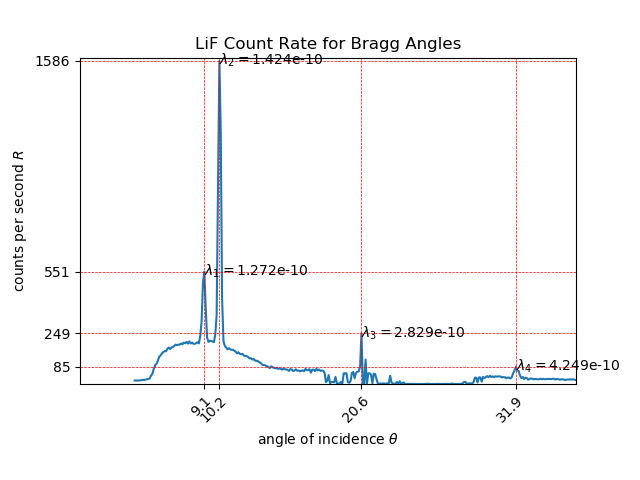
\includegraphics{LiF1}
\end{figure}

\begin{figure}[h]
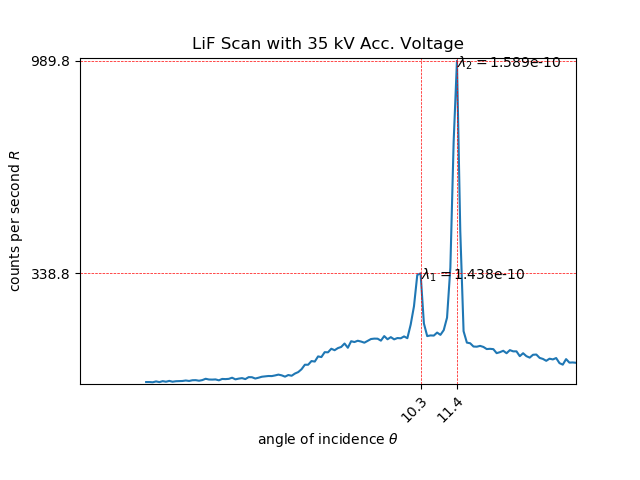
\includegraphics{ve1}
\end{figure}

\begin{figure}[h]
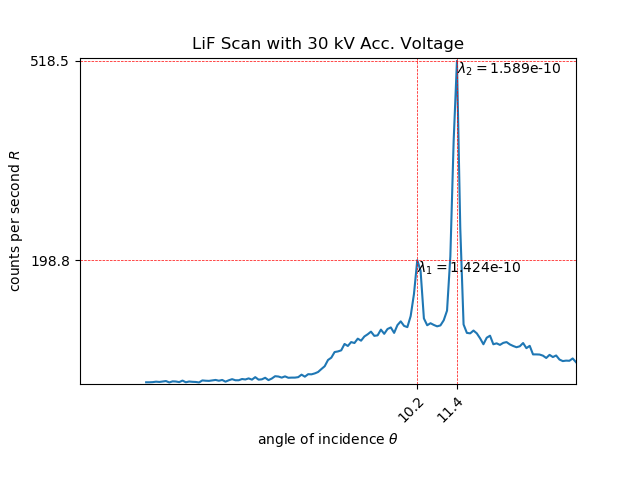
\includegraphics{ve2}
\end{figure}

\begin{figure}[h]
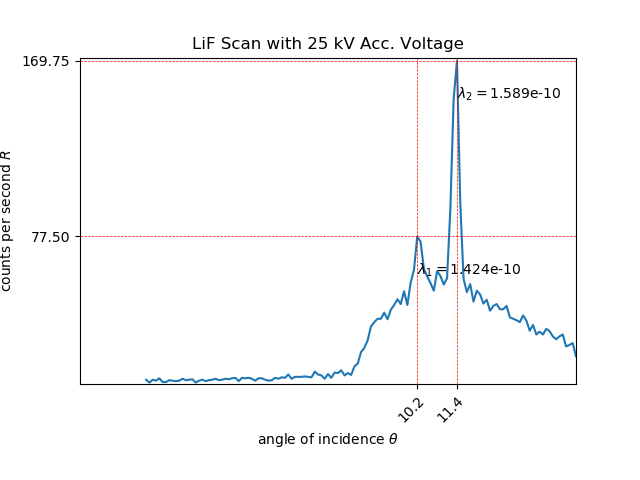
\includegraphics{ve3}
\end{figure}

\begin{figure}[h]
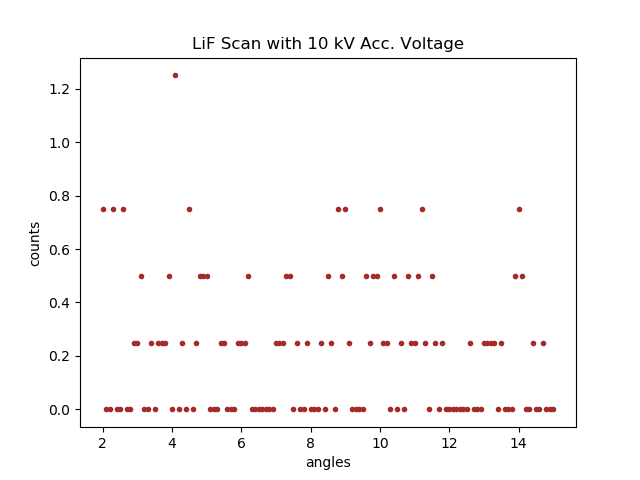
\includegraphics{ve4}
\end{figure}

\begin{figure}[h]
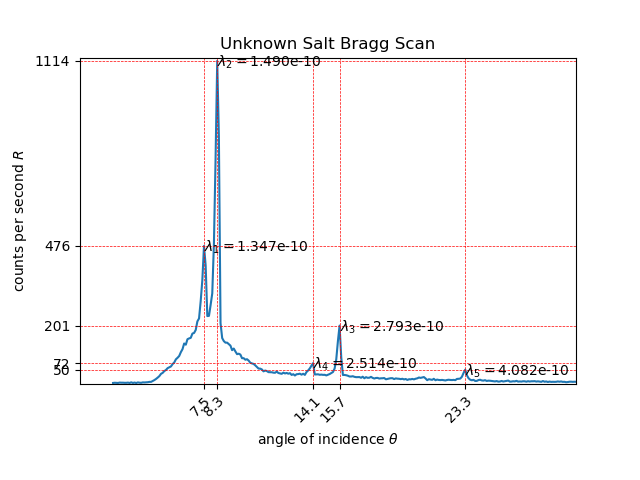
\includegraphics{uks1}
\end{figure}

\begin{figure}[h]
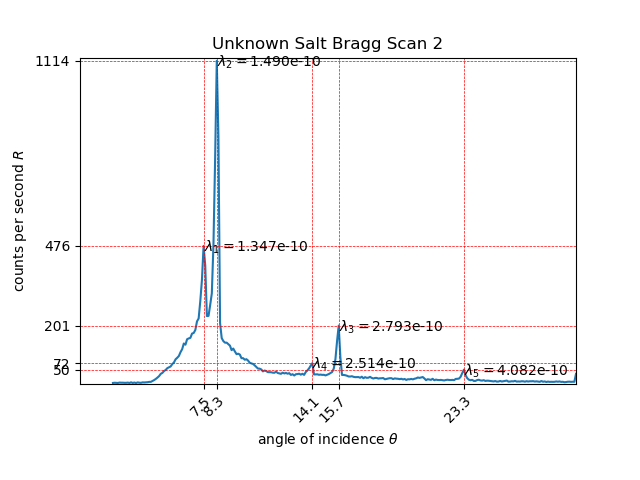
\includegraphics{uks2}
\end{figure}

\begin{figure}[h]
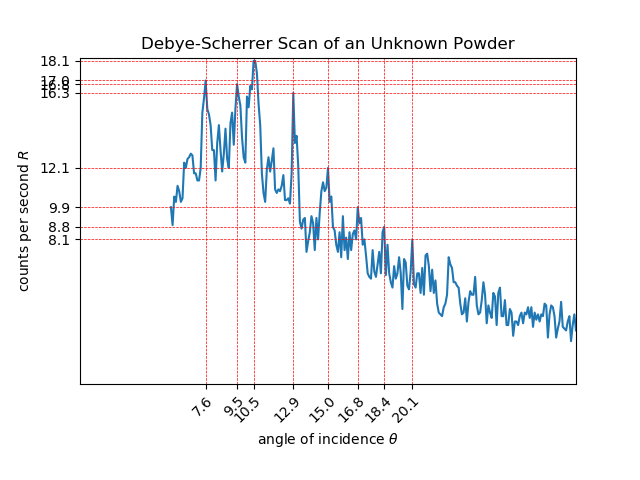
\includegraphics{ukp1}
\end{figure}

\begin{figure}[h]
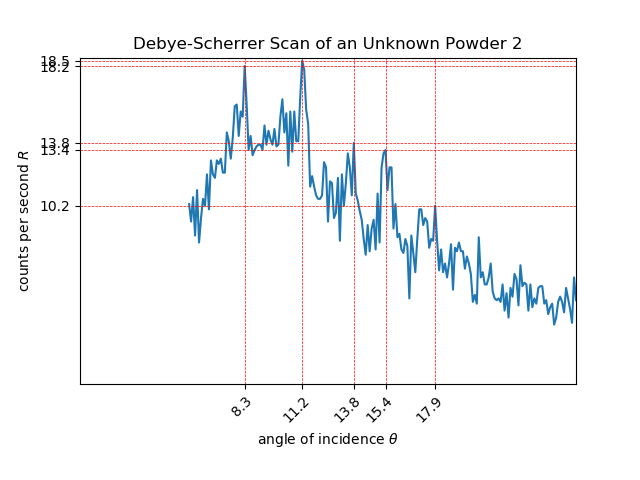
\includegraphics{ukp2}
\end{figure}

\begin{figure}[h]
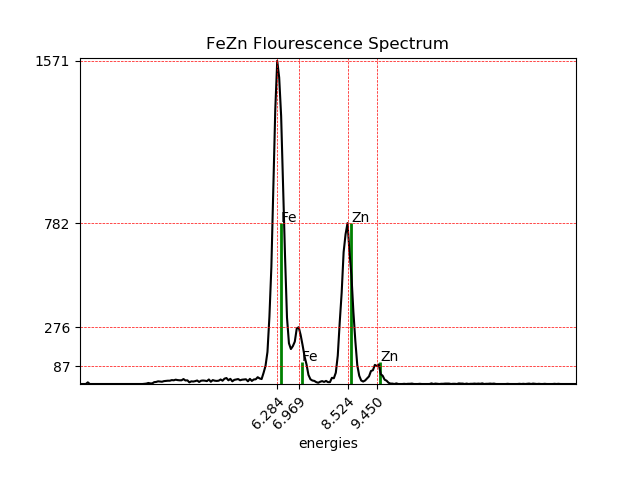
\includegraphics{fFeZn}
\end{figure}

\begin{figure}[h]
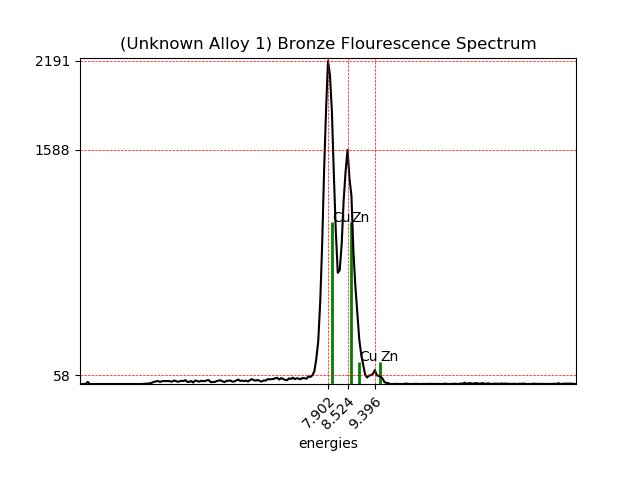
\includegraphics{fbronze}
\end{figure}

\begin{figure}[h]
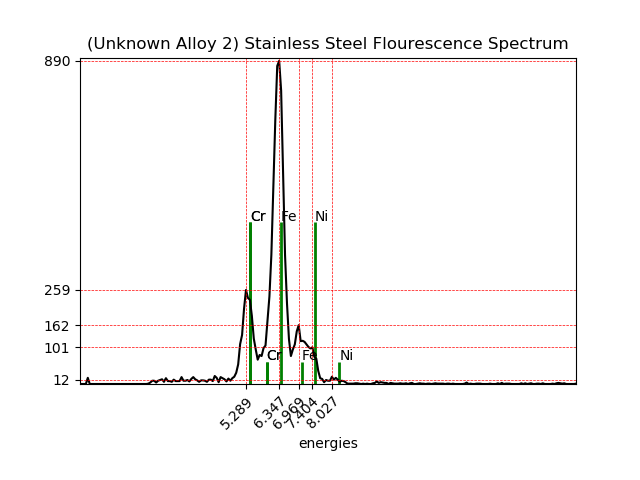
\includegraphics{fssteel}
\end{figure}

\begin{figure}[h]
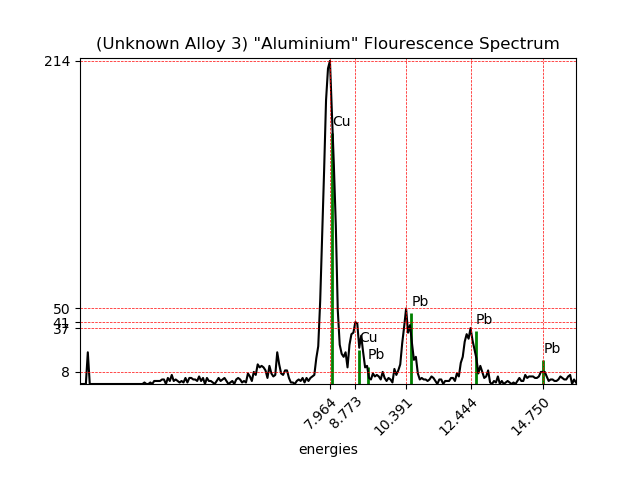
\includegraphics{fCuPb}
\end{figure}

\begin{figure}[h]
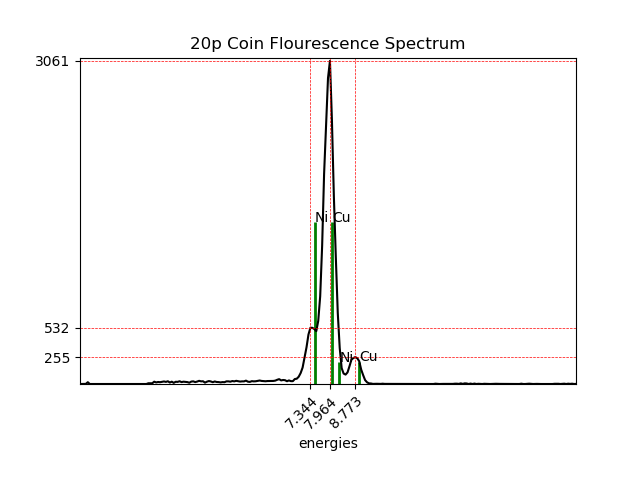
\includegraphics{f20p}
\end{figure}

\end{document}
